\documentclass[%preprint,
notitlepage,
%superscriptaddress,
%groupedaddress,
%unsortedaddress,
%runinaddress,
%frontmatterverbose, 
%preprint,
%preprintnumbers,
%nofootinbib,
%nobibnotes,
%bibnotes,
 amsmath,amssymb,
 aps,
%pra,
%prb,
rmp,
%prstab,
%prstper,
%floatfix,
]{revtex4-2}  % defines the basic parameters of the document

% if you want a single-column, remove reprint

% allows special characters (including æøå)
\usepackage[utf8]{inputenc}
\usepackage[norsk]{babel}

%% note that you may need to download some of these packages manually, it depends on your setup.
%% I recommend downloading TeXMaker, because it includes a large library of the most common packages.

\usepackage{physics,amssymb}  % mathematical symbols (physics imports amsmath)
\usepackage{graphicx}         % include graphics such as plots
\usepackage{xcolor}           % set colors
\usepackage{hyperref}         % automagic cross-referencing (this is GODLIKE)
\usepackage{tikz}             % draw figures manually
\usetikzlibrary{tikzmark}
\usepackage{listings}         % display code
\usepackage{subfigure}        % imports a lot of cool and useful figure commands
\usepackage{cprotect}
\usepackage{float}
\usepackage{caption}

\setlength{\parindent}{0px}

%Ta med disse kommandoene
\newcommand{\nnode}[2]{\node (#1) at (#2) {#1};}    %Her defineres nnode kommandoen
\newcommand{\relnode}[2]{\draw (#2) node[fill,circle,scale=0.6]{} (#2);\node (#1) at (#2) {};}  %Her defineres relnode kommandoen

% defines the color of hyperref objects
% Blending two colors:  blue!80!black  =  80% blue and 20% black
\hypersetup{ % this is just my personal choice, feel free to change things
    colorlinks,
    linkcolor={red!50!black},
    citecolor={blue!50!black},
    urlcolor={blue!80!black}}
%
%% Defines the style of the programming listing
%% This is actually my personal template, go ahead and change stuff if you want
\lstnewenvironment{python}{
	\lstset{ %
		inputpath=,
		backgroundcolor=\color{white!95!black},
		basicstyle={\ttfamily\scriptsize},
		commentstyle=\color{orange},
		language=Python,
		numbers=left,
		stepnumber=1,
		morekeywords={True,False},
		tabsize=4,
		stringstyle=\color{green!55!black},
		frame=single,
		keywordstyle=\color{blue},
		showstringspaces=false,
		columns=fullflexible,
		keepspaces=true}
}{}

\lstnewenvironment{cpp}{
	\lstset{ %
		inputpath=,
		backgroundcolor=\color{white!95!black},
		basicstyle={\ttfamily\scriptsize},
		commentstyle=\color{orange},
		language=C++,
		numbers=left,
		stepnumber=1,
		morekeywords={True,False},
		tabsize=4,
		stringstyle=\color{green!55!black},
		frame=single,
		keywordstyle=\color{blue},
		showstringspaces=false,
		columns=fullflexible,
		keepspaces=true}
}{}

\lstnewenvironment{sql}{
	\lstset{ %
		inputpath=,
		backgroundcolor=\color{white!95!black},
		basicstyle={\ttfamily\scriptsize},
		commentstyle=\color{orange},
		language=SQL,
		numbers=left,
		stepnumber=1,
		morekeywords={True,False},
		tabsize=4,
		stringstyle=\color{green!55!black},
		frame=single,
		keywordstyle=\color{blue},
		showstringspaces=false,
		columns=fullflexible,
		keepspaces=true}
}{}

\lstset{literate=
  {á}{{\'a}}1 {é}{{\'e}}1 {í}{{\'i}}1 {ó}{{\'o}}1 {ú}{{\'u}}1
  {Á}{{\'A}}1 {É}{{\'E}}1 {Í}{{\'I}}1 {Ó}{{\'O}}1 {Ú}{{\'U}}1
  {à}{{\`a}}1 {è}{{\`e}}1 {ì}{{\`i}}1 {ò}{{\`o}}1 {ù}{{\`u}}1
  {À}{{\`A}}1 {È}{{\'E}}1 {Ì}{{\`I}}1 {Ò}{{\`O}}1 {Ù}{{\`U}}1
  {ä}{{\"a}}1 {ë}{{\"e}}1 {ï}{{\"i}}1 {ö}{{\"o}}1 {ü}{{\"u}}1
  {Ä}{{\"A}}1 {Ë}{{\"E}}1 {Ï}{{\"I}}1 {Ö}{{\"O}}1 {Ü}{{\"U}}1
  {â}{{\^a}}1 {ê}{{\^e}}1 {î}{{\^i}}1 {ô}{{\^o}}1 {û}{{\^u}}1
  {Â}{{\^A}}1 {Ê}{{\^E}}1 {Î}{{\^I}}1 {Ô}{{\^O}}1 {Û}{{\^U}}1
  {œ}{{\oe}}1 {Œ}{{\OE}}1 {æ}{{\ae}}1 {Æ}{{\AE}}1 {ß}{{\ss}}1
  {ű}{{\H{u}}}1 {Ű}{{\H{U}}}1 {ő}{{\H{o}}}1 {Ő}{{\H{O}}}1
  {ç}{{\c c}}1 {Ç}{{\c C}}1 {ø}{{\o}}1 {å}{{\r a}}1 {Å}{{\r A}}1
  {€}{{\euro}}1 {£}{{\pounds}}1 {«}{{\guillemotleft}}1
  {»}{{\guillemotright}}1 {ñ}{{\~n}}1 {Ñ}{{\~N}}1 {¿}{{?`}}1
}

\newcommand{\set}[1]{\ensuremath{\left\{#1\right\}}}
\newcommand{\tuple}[1]{\ensuremath{\left\langle #1 \right\rangle}}
\newcommand{\imp}{\ensuremath{\rightarrow}}

\newcommand{\ceil}[1]{\ensuremath{\lceil #1 \rceil}}
\newcommand{\floor}[1]{\ensuremath{\lfloor #1 \rfloor}}

\usepackage{thmtools}
\DeclareMathOperator{\nullspace}{Nul}
\DeclareMathOperator{\collspace}{Col}
\DeclareMathOperator{\rref}{Rref}
%%\DeclareMathOperator{\dim}{Dim}

 % "meq": must be equal
\newcommand{\meq}{\overset{!}{=}}
\newcommand\numberthis{\addtocounter{equation}{1}\tag{\theequation}}

\newcommand{\R}{\mathbb{R}}
\newcommand{\N}{\mathbb{N}}
\newcommand{\Z}{\mathbb{Z}}
\newcommand{\Q}{\mathbb{Q}}
\newcommand{\C}{\mathbb{C}}
\newcommand*\Heq{\ensuremath{\overset{\kern2pt L'H}{=}}}
\usepackage{bm}
\newcommand{\uveci}{{\bm{\hat{\textnormal{\bfseries\i}}}}}
\newcommand{\uvecj}{{\bm{\hat{\textnormal{\bfseries\j}}}}}
\DeclareRobustCommand{\uvec}[1]{{%
  \ifcsname uvec#1\endcsname
     \csname uvec#1\endcsname
   \else
    \bm{\hat{\mathbf{#1}}}%
   \fi
}}
\usepackage[binary-units=true]{siunitx}

\newcommand{\twopartdef}[4]
{
	\left\{
		\begin{array}{ll}
			#1 & \mbox{if } #2 \\
			#3 & \mbox{if } #4
		\end{array}
	\right.
}

\makeatletter
\newcommand*{\balancecolsandclearpage}{%
  \close@column@grid
  \cleardoublepage
  \twocolumngrid
}
\makeatother

\AtBeginEnvironment{align}{\setcounter{equation}{0}}
\newcounter{subproject}
\renewcommand{\thesubproject}{\alph{subproject}}
\newenvironment{subproj}{
\begin{description}
	\item[\refstepcounter{subproject}(\thesubproject)]
}{\end{description}}


\begin{document}
\title{Oblig 1}   % self-explanatory
\author{Anders P. Åsbø}               % self-explanatory
\date{\today}                             % self-explanatory
\noaffiliation                            % ignore this

\maketitle                                % creates the title, author, date

\section*{Oppgave 1}
\subsection*{a)}
For å lage databasen "Oblig1" bruker jeg sql setningen
\begin{sql}
oblig1> CREATE SCHEMA Oblig1
[2022-09-11 16:51:14] 1 row affected in 9 ms
\end{sql}
Som resulterer i
\begin{figure}[H]
\centering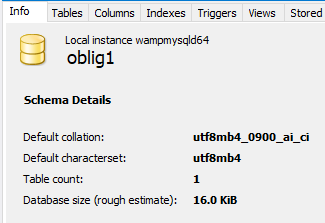
\includegraphics[scale=1]{op1a.png}
\end{figure}

\subsection*{b)}
For å lage tabellen "Film", så bruker jeg følgende sql:
\begin{sql}
oblig1> CREATE TABLE Oblig1.Film (
            FNr INTEGER UNSIGNED NOT NULL,
            Tittel VARCHAR(40) NOT NULL,
            År SMALLINT UNSIGNED,
            Land VARCHAR(40),
            Sjanger VARCHAR(20),
            Alder TINYINT UNSIGNED,
            Tid SMALLINT UNSIGNED,
            Pris DECIMAL(5, 2),
            PRIMARY KEY (FNr)
        )
[2022-09-11 17:25:37] completed in 19 ms
\end{sql}

\newpage
som resulterer i
\begin{figure}[H]
\centering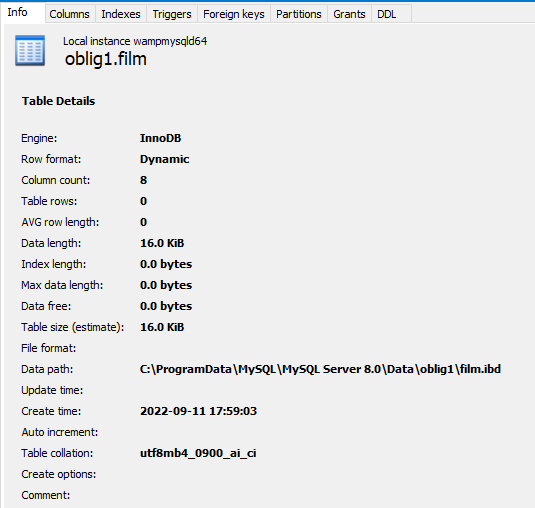
\includegraphics[scale=1]{op1b.png}
\end{figure}

\subsection*{c)}
Jeg legger til dataene fra tabellen i boken med følgende sql:
\begin{sql}
oblig1> INSERT INTO Oblig1.Film
        VALUES (1, 'Casablanca', 1942, 'USA', 'Drama', 15, 102, 149.00),
               (2, 'Fort Apachea', 1948, 'USA', 'Western', 15, 127, NULL),
               (3, 'Apocalypse Now', 1979, 'USA', 'Action', 18, 155, 123.00),
               (4, 'Streets of Fire', 1984, 'USA', 'Action', 15, 93, NULL),
               (5, 'High Noon', 1952, 'USA', 'Western', 15, 85, 123.00),
               (6, 'Cinema Paradiso', 1988, 'Italia', 'Komedie', 11, 123, NULL),
               (7, 'Asterix hos britene', 1988, 'Frankrike', 'Tegnefilm', 7, 78, 149.00),
               (8, 'Veiviseren', 1987, 'Norge', 'Action', 15, 96, 87.00),
               (9, 'Salmer fra kjøkkenet', 2002, 'Norge', 'Komedie', 7, 80, 149.00),
               (10, 'Anastasia', 1997, 'USA', 'Tegnefilm', 7, 94, 123.00),
               (11, 'La Grande bouffe', 1973, 'Frankrike', 'Drama', 15, 129, 87.00),
               (12, 'Blues Brothers 2000', 1998, 'USA', 'Komedie', 11, 124, 135.00),
               (13, 'Beatles: Help', 1965, 'Storbritannia', 'Musikk', 11, 144, NULL)
[2022-09-11 18:13:34] 13 rows affected in 6 ms
oblig1> SELECT * FROM Oblig1.Film
[2022-09-11 18:19:18] 13 rows retrieved starting from 1 in 39 ms (execution: 5 ms, fetching: 34 ms)
\end{sql}

\newpage
som resulterer i
\begin{figure}[H]
\centering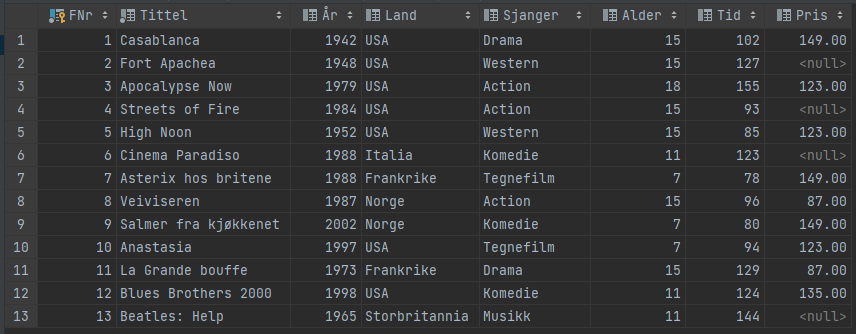
\includegraphics[width=\columnwidth]{op1c.png}
\end{figure}

\subsection*{d)}
For å finne tittel, sjanger og pris for filmer produsert i eller etter 1988, og sortere resultatet synkende etter pris, så bruker jeg følgende spørring:
\begin{sql}
oblig1> SELECT Tittel, Sjanger, Pris
        FROM Oblig1.Film
        WHERE År >= 1988
        ORDER BY Pris DESC
[2022-09-11 18:13:38] 5 rows retrieved starting from 1 in 44 ms (execution: 5 ms, fetching: 39 ms)
\end{sql}
som resulterer i
\begin{figure}[H]
\centering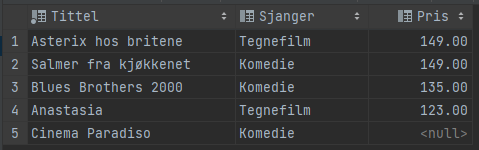
\includegraphics[scale=1]{op1d.png}
\end{figure}

\subsection*{e)}
For å hente alle kolonner for filmer som mangler pris, sortert først etter aldersgrense og så alfabetisk etter sjanger, så bruker jeg følgende spørring:
\begin{sql}
oblig1> SELECT * FROM Oblig1.Film
        WHERE Pris IS NULL
        ORDER BY Alder, Sjanger ASC
[2022-09-11 18:26:48] 4 rows retrieved starting from 1 in 52 ms (execution: 18 ms, fetching: 34 ms)
\end{sql}
\newpage
som resulterer i
\begin{figure}[H]
\centering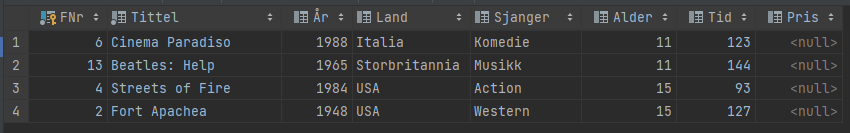
\includegraphics[width=\columnwidth]{op1e.png}
\end{figure}

\subsection*{f)}
Jeg finner antall filmer i hver sjanger som er til salgs, og totalpris per sjanger, ved hjelp av følgende spørring:
\begin{sql}
oblig1> SELECT Sjanger, COUNT(Sjanger) AS 'Antall filmer', SUM(Pris) AS 'Totalpris'
        FROM Oblig1.Film
        WHERE Pris IS NOT NULL
        GROUP BY Sjanger
        ORDER BY Sjanger ASC
[2022-09-11 18:51:56] 5 rows retrieved starting from 1 in 30 ms (execution: 5 ms, fetching: 25 ms)
\end{sql}
som resulterer i
\begin{figure}[H]
\centering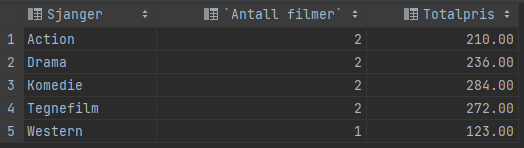
\includegraphics[width=\columnwidth]{op1f.png}
\end{figure}

\subsection*{g)}
Jeg legger til data for filmen "Ghost in the Shell (1995)" ved følgende spørring:
\begin{sql}
oblig1> INSERT INTO Oblig1.Film
        VALUE (14, 'Ghost in the Shell', 1995, 'Japan', 'Tegnefilm', 13, 83, 95.00)
[2022-09-11 19:02:07] 1 row affected in 19 ms
oblig1> SELECT * FROM Oblig1.Film
        WHERE Tittel = 'Ghost in the Shell'
[2022-09-11 19:04:31] 1 row retrieved starting from 1 in 29 ms (execution: 4 ms, fetching: 25 ms)
\end{sql}
som resulterer i
\begin{figure}[H]
\centering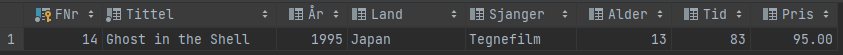
\includegraphics[width=\columnwidth]{op1g.png}
\end{figure}

\newpage
\subsection*{h)}
Bruker følgende sql for å korrigere tittelen film nummer \(5\) fra 'High Noon' til 'High Moon':
\begin{sql}
oblig1> UPDATE Oblig1.Film
        SET Tittel = 'High Moon'
        WHERE Tittel = 'High Noon'
[2022-09-11 19:15:28] 1 row affected in 7 ms
oblig1> SELECT FNr, Tittel
        FROM Oblig1.Film
        WHERE Tittel = 'High Moon'
[2022-09-11 19:16:32] 1 row retrieved starting from 1 in 30 ms (execution: 5 ms, fetching: 25 ms)
\end{sql}
som resulterer i
\begin{figure}[H]
\centering
\includegraphics[scale=1]{op1h.png}
\end{figure}

\subsection*{i)}
Øker prisen med \(10\%\) på action-filmer med følgende kode:
\begin{sql}
oblig1> UPDATE Oblig1.Film
        SET Pris = Pris * 1.1
        WHERE Sjanger = 'Action'
[2022-09-11 19:23:18] 3 rows affected in 6 ms
oblig1> SELECT Sjanger, Tittel, Pris
        FROM Oblig1.Film
        WHERE Sjanger = 'Action'
        ORDER BY Tittel ASC
[2022-09-11 19:27:54] 3 rows retrieved starting from 1 in 31 ms (execution: 4 ms, fetching: 27 ms)
\end{sql}
som resulterer i
\begin{figure}[H]
\centering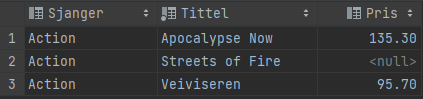
\includegraphics[scale=1]{op1i.png}
\end{figure}

\section*{j}
Sletter filmen 'Anastasia':
\begin{sql}
oblig1> DELETE
        FROM Oblig1.Film
        WHERE Tittel = 'Anastasia'
[2022-09-11 19:34:24] 1 row affected in 21 ms
oblig1> SELECT Tittel
        FROM Oblig1.Film
        ORDER BY Tittel ASC
[2022-09-11 19:35:25] 13 rows retrieved starting from 1 in 35 ms (execution: 17 ms, fetching: 18 ms)
\end{sql}
\newpage
som resulterer i
\begin{figure}[H]
\centering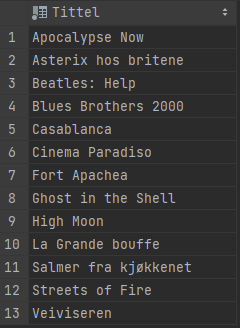
\includegraphics[scale=1]{op1j.png}
\end{figure}

\section*{Oppgave 2}
\subsection*{a)}
Lager tabellen 'Kunde':
\begin{sql}
oblig1> CREATE TABLE Oblig1.Kunde (
            KNr INTEGER UNSIGNED NOT NULL,
            Fornavn VARCHAR(50),
            Etternavn VARCHAR(50),
            Adresse VARCHAR(100),
            PostNr SMALLINT UNSIGNED,
            PRIMARY KEY (KNr)
        )
[2022-09-11 19:45:51] completed in 37 ms
oblig1> SELECT *
        FROM Oblig1.kunde
[2022-09-11 19:47:38] 0 rows retrieved in 29 ms (execution: 4 ms, fetching: 25 ms)
\end{sql}
som resulterer i
\begin{figure}[H]
\centering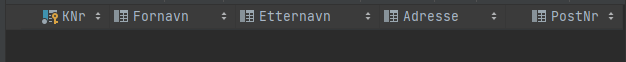
\includegraphics[scale=1]{op2a.png}
\end{figure}

\subsection*{b)}
Legger til data for tre kunder:
\begin{sql}
oblig1> INSERT INTO Oblig1.Kunde
        VALUES (10001, 'Kari', 'Mo', 'Moldegata 21 H0402', 0445),
               (10002, 'Geir', 'Gallestein', 'Grønnegata 68 H0304', 2317),
               (10003, 'Reidun', 'Roterud', 'Hylleråsvegen 11', 2440)
[2022-09-11 19:56:01] 3 rows affected in 6 ms
oblig1> SELECT *
        FROM Oblig1.Kunde
[2022-09-11 19:56:03] 3 rows retrieved starting from 1 in 35 ms (execution: 5 ms, fetching: 30 ms)
\end{sql}
som resulterer i
\begin{figure}[H]
\centering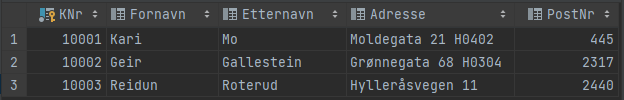
\includegraphics[width=\columnwidth]{op2b.png}
\end{figure}

\end{document}